\documentclass[ddcfooter]{tudbeamer}
\usepackage{german}
\begin{document}
\einrichtung{Fakult"at Informatik}
%\institut{Institut f"ur XXX}
\title[Informatik und Gesellschaft]{Informatik und Gesellschaft}
%\subtitle{\ldots in der auch wieder Goethe zitiert wird.}
\author{Cheng Chen, Kaijun Chen, Xiaoyao Li, Jing Zheng, Junlin Huang}
\maketitle

\section{Einführung}
\begin{frame}
\frametitle{Einf"uhrung}
%\framesubtitle{hehe}
\begin{itemize}
\item Wie beeinflusst Bitcoin die Wirtschaft?
\item Thema 2
\item Thema 3
\item Thema 4
\end{itemize}
\end{frame}

%PART: Junlin Huang
%BEGIN
\section{Bitcoin}

%Eigentschaft von Bitcoin
\begin{frame}
\frametitle{Bitcoin}
\begin{itemize}
\item Kleines deflationäre Risiko
\item Bitcoin kann nicht gef"alscht werden
\item Bitcoin ist v"ollig dezentral
\end{itemize}
\end{frame}

\begin{frame}
\frametitle{Bitcoin}
\begin{itemize}
\item 111
\end{itemize}
\end{frame}

\begin{frame}
\frametitle{Bitcoin}
\begin{itemize}
\item Bitcoin kann unbegrenzt aufgeteilt werden
\begin{figure}
\centering
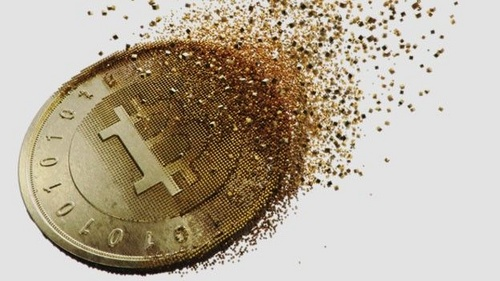
\includegraphics[height=3.5cm]{images/bitcoin_split}
\\http://img0.pconline.com.cn/pconline/1304/19/3263646\_11.jpg
\end{figure}

\end{itemize}
\end{frame}
%END

\section{Literatur}
\begin{frame}
\frametitle{Literatur}
\begin{itemize}
\item Goethe: Novelle. DB Sonderband: Meisterwerke deutscher Dichter und Denker, S. 12111 (vgl. Goethe-HA Bd. 6, S. 491)
\end{itemize}
\end{frame}

 \end{document}
